% RepNet-SE Architecture — Poster-quality figure
% Compile: pdflatex repnet_se_architecture.tex
\documentclass[border=14pt]{standalone}
\usepackage[T1]{fontenc}
\usepackage{lmodern}
\usepackage{amsmath}
\usepackage{tikz}
\usepackage{xcolor}
\usetikzlibrary{
  arrows.meta, calc, positioning, fit, backgrounds,
  shapes.geometric
}

% ── Vibrant palette ──
\definecolor{convblue}{HTML}{2563EB}
\definecolor{seorange}{HTML}{D97706}
\definecolor{attnviolet}{HTML}{7C3AED}
\definecolor{fusiongreen}{HTML}{059669}
\definecolor{poolslate}{HTML}{64748B}
\definecolor{textdark}{HTML}{1E293B}
\definecolor{textmid}{HTML}{64748B}
\definecolor{bordergray}{HTML}{94A3B8}
\definecolor{stagebg1}{HTML}{DBEAFE}
\definecolor{stagebg2}{HTML}{EDE9FE}
\definecolor{stagebg3}{HTML}{DBEAFE}
\definecolor{fusionbg}{HTML}{D1FAE5}

\tikzset{
  % Main flow blocks — bold fills
  block/.style={
    draw=#1, fill=#1!18, rounded corners=5pt,
    minimum height=0.95cm, minimum width=5.4cm,
    font=\small\sffamily, text=textdark,
    inner sep=5pt, line width=1pt,
  },
  % Sub-blocks inside stages — strong color identity
  conv/.style={
    draw=convblue, fill=convblue!22, rounded corners=4pt,
    minimum height=0.85cm, minimum width=4.6cm,
    font=\small\sffamily, text=textdark,
    inner sep=4pt, line width=0.9pt,
  },
  se/.style={
    draw=seorange, fill=seorange!22, rounded corners=4pt,
    minimum height=0.85cm, minimum width=4.6cm,
    font=\small\sffamily, text=textdark,
    inner sep=4pt, line width=0.9pt,
  },
  attn/.style={
    draw=attnviolet, fill=attnviolet!18, rounded corners=4pt,
    minimum height=0.85cm, minimum width=5.0cm,
    font=\small\sffamily, text=textdark,
    inner sep=4pt, line width=0.9pt,
  },
  pool/.style={
    draw=poolslate, fill=poolslate!10, rounded corners=4pt,
    minimum height=0.8cm, minimum width=4.6cm,
    font=\small\sffamily, text=textdark,
    inner sep=4pt, line width=0.7pt,
  },
  fuse/.style={
    draw=fusiongreen, fill=fusiongreen!20, rounded corners=4pt,
    minimum height=0.95cm, minimum width=5.0cm,
    font=\small\sffamily, text=textdark,
    inner sep=5pt, line width=1pt,
  },
  % Multi-scale branch boxes
  branch/.style={
    draw=convblue!80, fill=convblue!25, rounded corners=3pt,
    minimum height=0.7cm, minimum width=1.7cm,
    font=\footnotesize\sffamily\bfseries, text=textdark,
    inner sep=3pt, line width=0.8pt,
  },
  mpbranch/.style={
    draw=poolslate!80, fill=poolslate!18, rounded corners=3pt,
    minimum height=0.7cm, minimum width=1.7cm,
    font=\footnotesize\sffamily\bfseries, text=textdark,
    inner sep=3pt, line width=0.8pt,
  },
  % Stage container
  stage/.style={
    draw=bordergray!60, fill=#1, rounded corners=9pt,
    inner sep=11pt, line width=0.5pt,
  },
  % Decomposition panel (right side)
  panel/.style={
    draw=#1!60, fill=#1!8, rounded corners=7pt,
    inner sep=9pt, line width=1.2pt,
  },
  panelnode/.style={
    draw=#1!50, fill=#1!15, rounded corners=3pt,
    minimum width=4.4cm, minimum height=0.55cm,
    font=\footnotesize\sffamily, text=textdark,
    inner sep=3pt, line width=0.6pt,
  },
  % Arrows
  arr/.style={-{Stealth[length=5pt, width=4pt]}, line width=1pt, textdark!70},
  skiparr/.style={-{Stealth[length=4pt, width=3pt]}, line width=0.8pt,
                  dashed, poolslate},
  panelarr/.style={-{Stealth[length=3pt]}, line width=0.5pt, #1!40},
  % Labels
  stagelabel/.style={font=\sffamily\bfseries\small, text=textdark},
  dimtext/.style={font=\scriptsize\sffamily, text=textmid},
  paneltitle/.style={font=\sffamily\bfseries\small, text=#1},
}

\begin{document}
\begin{tikzpicture}[node distance=0.6cm]

% ════════════════════════════════════
%  INPUT
% ════════════════════════════════════

\node[draw=textdark!60, fill=textdark!8, rounded corners=5pt,
      minimum height=0.95cm, minimum width=4.2cm,
      font=\small\sffamily\bfseries, text=textdark, line width=1pt]
  (input) {12-Lead ECG};
\node[dimtext, right=0.4cm of input] {$(B,\;12,\;T)$};


% ════════════════════════════════════
%  STAGE 1
% ════════════════════════════════════

\node[branch, below=1.5cm of input, xshift=-2.7cm] (b1) {DW $k\!=\!5$};
\node[branch, right=0.3cm of b1]                   (b2) {DW $k\!=\!9$};
\node[branch, right=0.3cm of b2]                   (b3) {DW $k\!=\!15$};
\node[mpbranch, right=0.3cm of b3]                  (b4) {MaxPool};

\node[conv, below=0.65cm of $(b2)!0.5!(b3)$, minimum width=5.6cm]
  (concat) {Concat $\to$ Project $1\!\times\!1$ $\to$ BN};
\node[dimtext, right=0.3cm of concat] {$\to 16$ ch};

\node[se, below=0.45cm of concat] (se1) {Squeeze-and-Excitation};

\node[pool, below=0.45cm of se1]
  (pool1) {GELU $\to$ MaxPool(2) $\to$ Dropout};

\node[attn, below=0.45cm of pool1, minimum width=5.6cm]
  (cla1) {Cross-Lead Attention};
\node[dimtext, right=0.3cm of cla1] {4 heads};

% Stage 1 arrows
\foreach \b in {b1, b2, b3, b4} {
  \draw[arr] (input.south) -- ++(0,-0.5) -| (\b.north);
}
\foreach \b in {b1, b2, b3, b4} {
  \draw[arr] (\b.south) -- ++(0,-0.15) -| (concat.north);
}
\draw[arr] (concat) -- (se1);
\draw[arr] (se1) -- (pool1);
\draw[arr] (pool1) -- (cla1);

% Stage 1 background
\begin{scope}[on background layer]
  \node[stage=stagebg1, fit=(b1)(b4)(cla1),
        minimum width=11cm] (s1bg) {};
\end{scope}
\node[stagelabel, anchor=north east] at ([xshift=-8pt, yshift=-4pt]s1bg.north west)
  {Stage 1 \textcolor{textmid}{\normalfont\small — Multi-Scale Inception + SE + Attention}};
\node[dimtext, anchor=south east] at ([yshift=4pt]s1bg.north east) {$1 \to 16$ channels};


% ════════════════════════════════════
%  STAGE 2
% ════════════════════════════════════

\node[conv, below=1.4cm of cla1] (conv2) {$2\times$ DSConv$(16\!\to\!32,\; k\!=\!5)$};
\node[se, below=0.35cm of conv2] (se2) {SE Block};
\node[pool, below=0.35cm of se2]
  (pool2) {Skip + GELU + Pool(2) + Dropout};
\node[attn, below=0.35cm of pool2] (cla2) {Cross-Lead Attention};
\node[dimtext, right=0.3cm of cla2] {4 heads};

\draw[skiparr] (conv2.west) -- ++(-0.55,0) |- (pool2.west);
\draw[arr] (cla1) -- (conv2);
\draw[arr] (conv2) -- (se2);
\draw[arr] (se2) -- (pool2);
\draw[arr] (pool2) -- (cla2);

\begin{scope}[on background layer]
  \node[stage=stagebg2, fit=(conv2)(cla2),
        minimum width=8.5cm] (s2bg) {};
\end{scope}
\node[stagelabel, anchor=north east] at ([xshift=-8pt, yshift=-4pt]s2bg.north west)
  {Stage 2 \textcolor{textmid}{\normalfont\small — SE Per-Lead Block + Cross-Lead Attention}};
\node[dimtext, anchor=south east] at ([yshift=4pt]s2bg.north east) {$16 \to 32$ channels};


% ════════════════════════════════════
%  STAGE 3
% ════════════════════════════════════

\node[conv, below=1.4cm of cla2] (conv3) {$2\times$ DSConv$(32\!\to\!64,\; k\!=\!5)$};
\node[se, below=0.35cm of conv3] (se3) {SE Block};
\node[pool, below=0.35cm of se3]
  (pool3) {Skip + GELU + Pool(2) + Dropout};
\node[attn, below=0.35cm of pool3] (cla3) {Cross-Lead Attention};
\node[dimtext, right=0.3cm of cla3] {4 heads};

\draw[skiparr] (conv3.west) -- ++(-0.55,0) |- (pool3.west);
\draw[arr] (cla2) -- (conv3);
\draw[arr] (conv3) -- (se3);
\draw[arr] (se3) -- (pool3);
\draw[arr] (pool3) -- (cla3);

\begin{scope}[on background layer]
  \node[stage=stagebg3, fit=(conv3)(cla3),
        minimum width=8.5cm] (s3bg) {};
\end{scope}
\node[stagelabel, anchor=north east] at ([xshift=-8pt, yshift=-4pt]s3bg.north west)
  {Stage 3 \textcolor{textmid}{\normalfont\small — SE Per-Lead Block + Cross-Lead Attention}};
\node[dimtext, anchor=south east] at ([yshift=4pt]s3bg.north east) {$32 \to 64$ channels};


% ════════════════════════════════════
%  CLASSIFICATION HEAD
% ════════════════════════════════════

\node[fuse, below=1.4cm of cla3] (gap) {Per-Lead Global Average Pooling};
\node[dimtext, right=0.3cm of gap] {$(B,\;12,\;64)$};

\node[fuse, below=0.5cm of gap, minimum width=5.6cm, line width=1.2pt,
      font=\small\sffamily\bfseries]
  (leadpool) {Lead Attention Pool};
\node[dimtext, right=0.3cm of leadpool] {$(B,\;64)$};

\node[draw=textdark!50, fill=textdark!8, rounded corners=4pt,
      minimum height=0.85cm, minimum width=4.0cm,
      font=\small\sffamily, text=textdark, line width=0.8pt,
      below=0.5cm of leadpool]
  (head) {Dropout(0.15) $\to$ Linear$(64\!\to\!2)$};

\node[draw=textdark!70, fill=textdark!12, rounded corners=5pt,
      minimum height=0.95cm, minimum width=3.6cm,
      font=\small\sffamily\bfseries, text=textdark, line width=1pt,
      below=0.5cm of head]
  (out) {$P(\text{preeclampsia})$};

\draw[arr] (cla3) -- (gap);
\draw[arr] (gap) -- (leadpool);
\draw[arr] (leadpool) -- (head);
\draw[arr] (head) -- (out);

\begin{scope}[on background layer]
  \node[stage=fusionbg, fit=(gap)(out)(leadpool)(head),
        minimum width=8.5cm] (fusbg) {};
\end{scope}
\node[stagelabel, anchor=north east] at ([xshift=-8pt, yshift=-4pt]fusbg.north west)
  {Classification Head \textcolor{textmid}{\normalfont\small — Lead Attention Pool + Linear}};


% ════════════════════════════════════
%  DECOMPOSITION PANELS (right side)
%  No callout arrows — color matching
%  links panels to main flow blocks
% ════════════════════════════════════

% Position panels aligned to right of stage backgrounds
\coordinate (panelanchor) at ([xshift=2.2cm]s1bg.north east);

% --- DSConv ---
\node[panel=convblue, anchor=north west, text width=5.6cm]
  at (panelanchor) (dscpanel) {
  {\sffamily\bfseries\small\color{convblue}Depthwise Separable Conv}
  \vspace{5pt}

  \begin{tikzpicture}[node distance=0.3cm]
    \node[panelnode=convblue] (dw)
      {Depthwise Conv (groups\,=\,$C_{\text{in}}$)};
    \node[panelnode=convblue, below=0.25cm of dw] (pw)
      {Pointwise $1\!\times\!1$ Conv};
    \draw[panelarr=convblue] (dw) -- (pw);
  \end{tikzpicture}

  \vspace{3pt}
  {\scriptsize\sffamily\color{textmid}
  Per-channel spatial filtering, then $1\!\times\!1$ channel mixing.
  Weights shared across all 12 leads.}
};

% --- SE Block ---
\node[panel=seorange, below=0.6cm of dscpanel.south west,
      anchor=north west, text width=5.6cm] (sepanel) {
  {\sffamily\bfseries\small\color{seorange}Squeeze-and-Excitation Block}
  \vspace{5pt}

  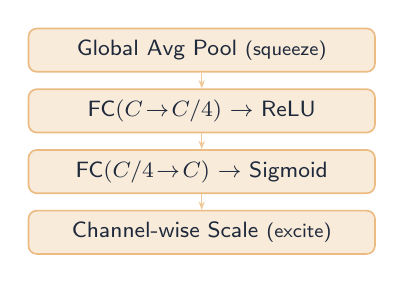
\begin{tikzpicture}[node distance=0.25cm]
    \node[panelnode=seorange] (sq)
      {Global Avg Pool {\scriptsize(squeeze)}};
    \node[panelnode=seorange, below=0.2cm of sq] (fc1)
      {FC$(C \!\to\! C/4)$ $\to$ ReLU};
    \node[panelnode=seorange, below=0.2cm of fc1] (fc2)
      {FC$(C/4 \!\to\! C)$ $\to$ Sigmoid};
    \node[panelnode=seorange, below=0.2cm of fc2] (sc)
      {Channel-wise Scale {\scriptsize(excite)}};
    \draw[panelarr=seorange] (sq) -- (fc1);
    \draw[panelarr=seorange] (fc1) -- (fc2);
    \draw[panelarr=seorange] (fc2) -- (sc);
  \end{tikzpicture}

  \vspace{3pt}
  {\scriptsize\sffamily\color{textmid}
  Learns per-channel importance. Reduction $r\!=\!4$.}
};

% --- Cross-Lead Attention ---
\node[panel=attnviolet, below=0.6cm of sepanel.south west,
      anchor=north west, text width=5.6cm] (clapanel) {
  {\sffamily\bfseries\small\color{attnviolet}Cross-Lead Attention}
  \vspace{5pt}

  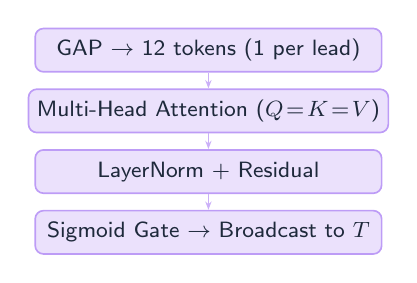
\begin{tikzpicture}[node distance=0.25cm]
    \node[panelnode=attnviolet] (tok)
      {GAP $\to$ 12 tokens (1 per lead)};
    \node[panelnode=attnviolet, below=0.2cm of tok] (mha)
      {Multi-Head Attention ($Q\!=\!K\!=\!V$)};
    \node[panelnode=attnviolet, below=0.2cm of mha] (ln)
      {LayerNorm + Residual};
    \node[panelnode=attnviolet, below=0.2cm of ln] (gate)
      {Sigmoid Gate $\to$ Broadcast to $T$};
    \draw[panelarr=attnviolet] (tok) -- (mha);
    \draw[panelarr=attnviolet] (mha) -- (ln);
    \draw[panelarr=attnviolet] (ln) -- (gate);
  \end{tikzpicture}

  \vspace{3pt}
  {\scriptsize\sffamily\color{textmid}
  Self-attention across 12 ECG leads with sigmoid gating.
  4 heads per stage.}
};

% --- Lead Attention Pool ---
\node[panel=fusiongreen, below=0.6cm of clapanel.south west,
      anchor=north west, text width=5.6cm] (lappanel) {
  {\sffamily\bfseries\small\color{fusiongreen}Lead Attention Pool}
  \vspace{5pt}

  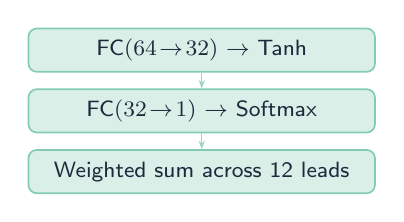
\begin{tikzpicture}[node distance=0.25cm]
    \node[panelnode=fusiongreen] (a1)
      {FC$(64 \!\to\! 32)$ $\to$ Tanh};
    \node[panelnode=fusiongreen, below=0.2cm of a1] (a2)
      {FC$(32 \!\to\! 1)$ $\to$ Softmax};
    \node[panelnode=fusiongreen, below=0.2cm of a2] (a3)
      {Weighted sum across 12 leads};
    \draw[panelarr=fusiongreen] (a1) -- (a2);
    \draw[panelarr=fusiongreen] (a2) -- (a3);
  \end{tikzpicture}

  \vspace{3pt}
  {\scriptsize\sffamily\color{textmid}
  Learns which leads are most informative per sample.}
};


% ════════════════════════════════════
%  FOOTER
% ════════════════════════════════════

\node[anchor=north, font=\small\sffamily, text=textdark,
      below=0.8cm of out] (footer) {
  \textbf{65,748 parameters}
  \;\textcolor{textmid}{\textbar}\ \
  Per-lead convolutions share weights across 12 leads
  \;\textcolor{textmid}{\textbar}\ \
  GELU activations throughout
};

% White background
\begin{scope}[on background layer]
  \fill[white] ([shift={(-5pt,-5pt)}]current bounding box.south west)
    rectangle ([shift={(5pt,5pt)}]current bounding box.north east);
\end{scope}

\end{tikzpicture}
\end{document}
